\documentclass{beamer}

\begin{document}

\begin{frame}
\frametitle{A doua lege a miscarii a lui Newton}
\end{frame}

\begin{frame}
\frametitle{ Analiza rezultatelor obtinute conform legii a doua a miscarii a lui Newton}
\begin{figure}
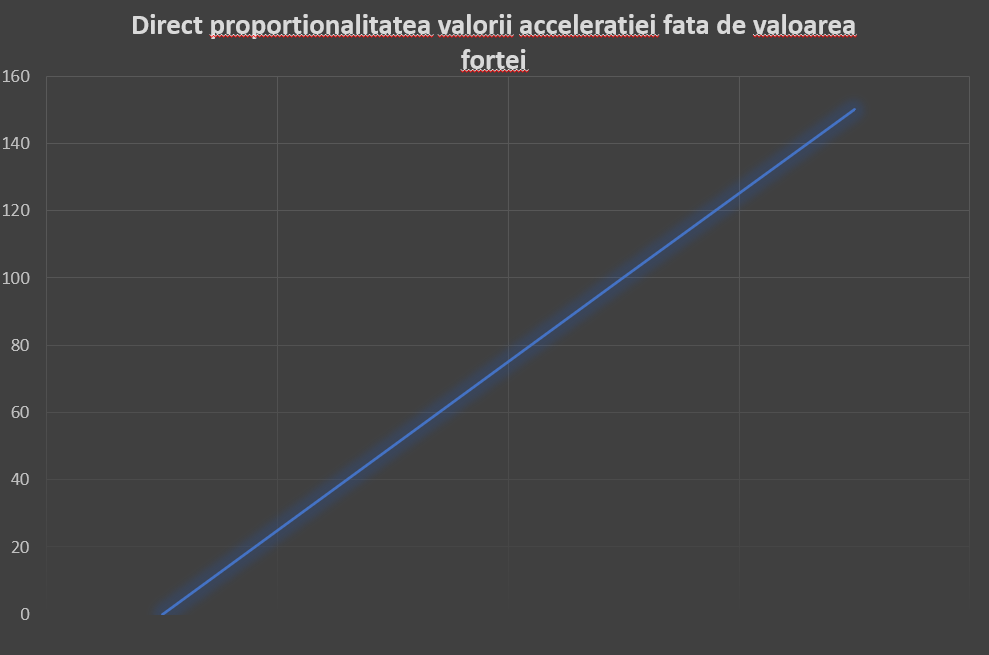
\includegraphics[width=\textwidth]{Picture1.png}
\end{figure}
\end{frame}

\begin{frame}
\frametitle{Tabel cu valori ale fortei si acceleratiei }
\begin{tabular}{|l|l|l|} \hline
Nr & Forta & Acceleratie \\ \hline
1 & 500 & 50  \\ \hline
2 & 1000 & 100  \\ \hline
3 & 1500 & 150  \\ \hline
4 & 2000 & 200  \\ \hline
5 & 2500 & 250  \\ \hline
6 & 3000 & 300  \\ \hline
7 & 3500 & 350  \\ \hline
8 & 4000 & 400  \\ \hline
\end{tabular}
\end{frame}
\begin{frame}
\frametitle{Concluzii}
A doua lege a mișcării a lui Newton a dovedit ca accelerația și forța sunt direct proporționale una față de cealaltă.
Aceasta a fost privită ca stabilind un nou program de cercetare pentru fizică.

\end{frame}

\end{document}